\documentclass[1p]{elsarticle_modified}
%\bibliographystyle{elsarticle-num}

%\usepackage[colorlinks]{hyperref}
%\usepackage{abbrmath_seonhwa} %\Abb, \Ascr, \Acal ,\Abf, \Afrak
\usepackage{amsfonts}
\usepackage{amssymb}
\usepackage{amsmath}
\usepackage{amsthm}
\usepackage{scalefnt}
\usepackage{amsbsy}
\usepackage{kotex}
\usepackage{caption}
\usepackage{subfig}
\usepackage{color}
\usepackage{graphicx}
\usepackage{xcolor} %% white, black, red, green, blue, cyan, magenta, yellow
\usepackage{float}
\usepackage{setspace}
\usepackage{hyperref}

\usepackage{tikz}
\usetikzlibrary{arrows}

\usepackage{multirow}
\usepackage{array} % fixed length table
\usepackage{hhline}

%%%%%%%%%%%%%%%%%%%%%
\makeatletter
\renewcommand*\env@matrix[1][\arraystretch]{%
	\edef\arraystretch{#1}%
	\hskip -\arraycolsep
	\let\@ifnextchar\new@ifnextchar
	\array{*\c@MaxMatrixCols c}}
\makeatother %https://tex.stackexchange.com/questions/14071/how-can-i-increase-the-line-spacing-in-a-matrix
%%%%%%%%%%%%%%%

\usepackage[normalem]{ulem}

\newcommand{\msout}[1]{\ifmmode\text{\sout{\ensuremath{#1}}}\else\sout{#1}\fi}
%SOURCE: \msout is \stkout macro in https://tex.stackexchange.com/questions/20609/strikeout-in-math-mode

\newcommand{\cancel}[1]{
	\ifmmode
	{\color{red}\msout{#1}}
	\else
	{\color{red}\sout{#1}}
	\fi
}

\newcommand{\add}[1]{
	{\color{blue}\uwave{#1}}
}

\newcommand{\replace}[2]{
	\ifmmode
	{\color{red}\msout{#1}}{\color{blue}\uwave{#2}}
	\else
	{\color{red}\sout{#1}}{\color{blue}\uwave{#2}}
	\fi
}

\newcommand{\Sol}{\mathcal{S}} %segment
\newcommand{\D}{D} %diagram
\newcommand{\A}{\mathcal{A}} %arc


%%%%%%%%%%%%%%%%%%%%%%%%%%%%%5 test

\def\sl{\operatorname{\textup{SL}}(2,\Cbb)}
\def\psl{\operatorname{\textup{PSL}}(2,\Cbb)}
\def\quan{\mkern 1mu \triangleright \mkern 1mu}

\theoremstyle{definition}
\newtheorem{thm}{Theorem}[section]
\newtheorem{prop}[thm]{Proposition}
\newtheorem{lem}[thm]{Lemma}
\newtheorem{ques}[thm]{Question}
\newtheorem{cor}[thm]{Corollary}
\newtheorem{defn}[thm]{Definition}
\newtheorem{exam}[thm]{Example}
\newtheorem{rmk}[thm]{Remark}
\newtheorem{alg}[thm]{Algorithm}

\newcommand{\I}{\sqrt{-1}}
\begin{document}

%\begin{frontmatter}
%
%\title{Boundary parabolic representations of knots up to 8 crossings}
%
%%% Group authors per affiliation:
%\author{Yunhi Cho} 
%\address{Department of Mathematics, University of Seoul, Seoul, Korea}
%\ead{yhcho@uos.ac.kr}
%
%
%\author{Seonhwa Kim} %\fnref{s_kim}}
%\address{Center for Geometry and Physics, Institute for Basic Science, Pohang, 37673, Korea}
%\ead{ryeona17@ibs.re.kr}
%
%\author{Hyuk Kim}
%\address{Department of Mathematical Sciences, Seoul National University, Seoul 08826, Korea}
%\ead{hyukkim@snu.ac.kr}
%
%\author{Seokbeom Yoon}
%\address{Department of Mathematical Sciences, Seoul National University, Seoul, 08826,  Korea}
%\ead{sbyoon15@snu.ac.kr}
%
%\begin{abstract}
%We find all boundary parabolic representation of knots up to 8 crossings.
%
%\end{abstract}
%\begin{keyword}
%    \MSC[2010] 57M25 
%\end{keyword}
%
%\end{frontmatter}

%\linenumbers
%\tableofcontents
%
\newcommand\colored[1]{\textcolor{white}{\rule[-0.35ex]{0.8em}{1.4ex}}\kern-0.8em\color{red} #1}%
%\newcommand\colored[1]{\textcolor{white}{ #1}\kern-2.17ex	\textcolor{white}{ #1}\kern-1.81ex	\textcolor{white}{ #1}\kern-2.15ex\color{red}#1	}

{\Large $\underline{12a_{0455}~(K12a_{0455})}$}

\setlength{\tabcolsep}{10pt}
\renewcommand{\arraystretch}{1.6}
\vspace{1cm}\begin{tabular}{m{100pt}>{\centering\arraybackslash}m{274pt}}
\multirow{5}{120pt}{
	\centering
	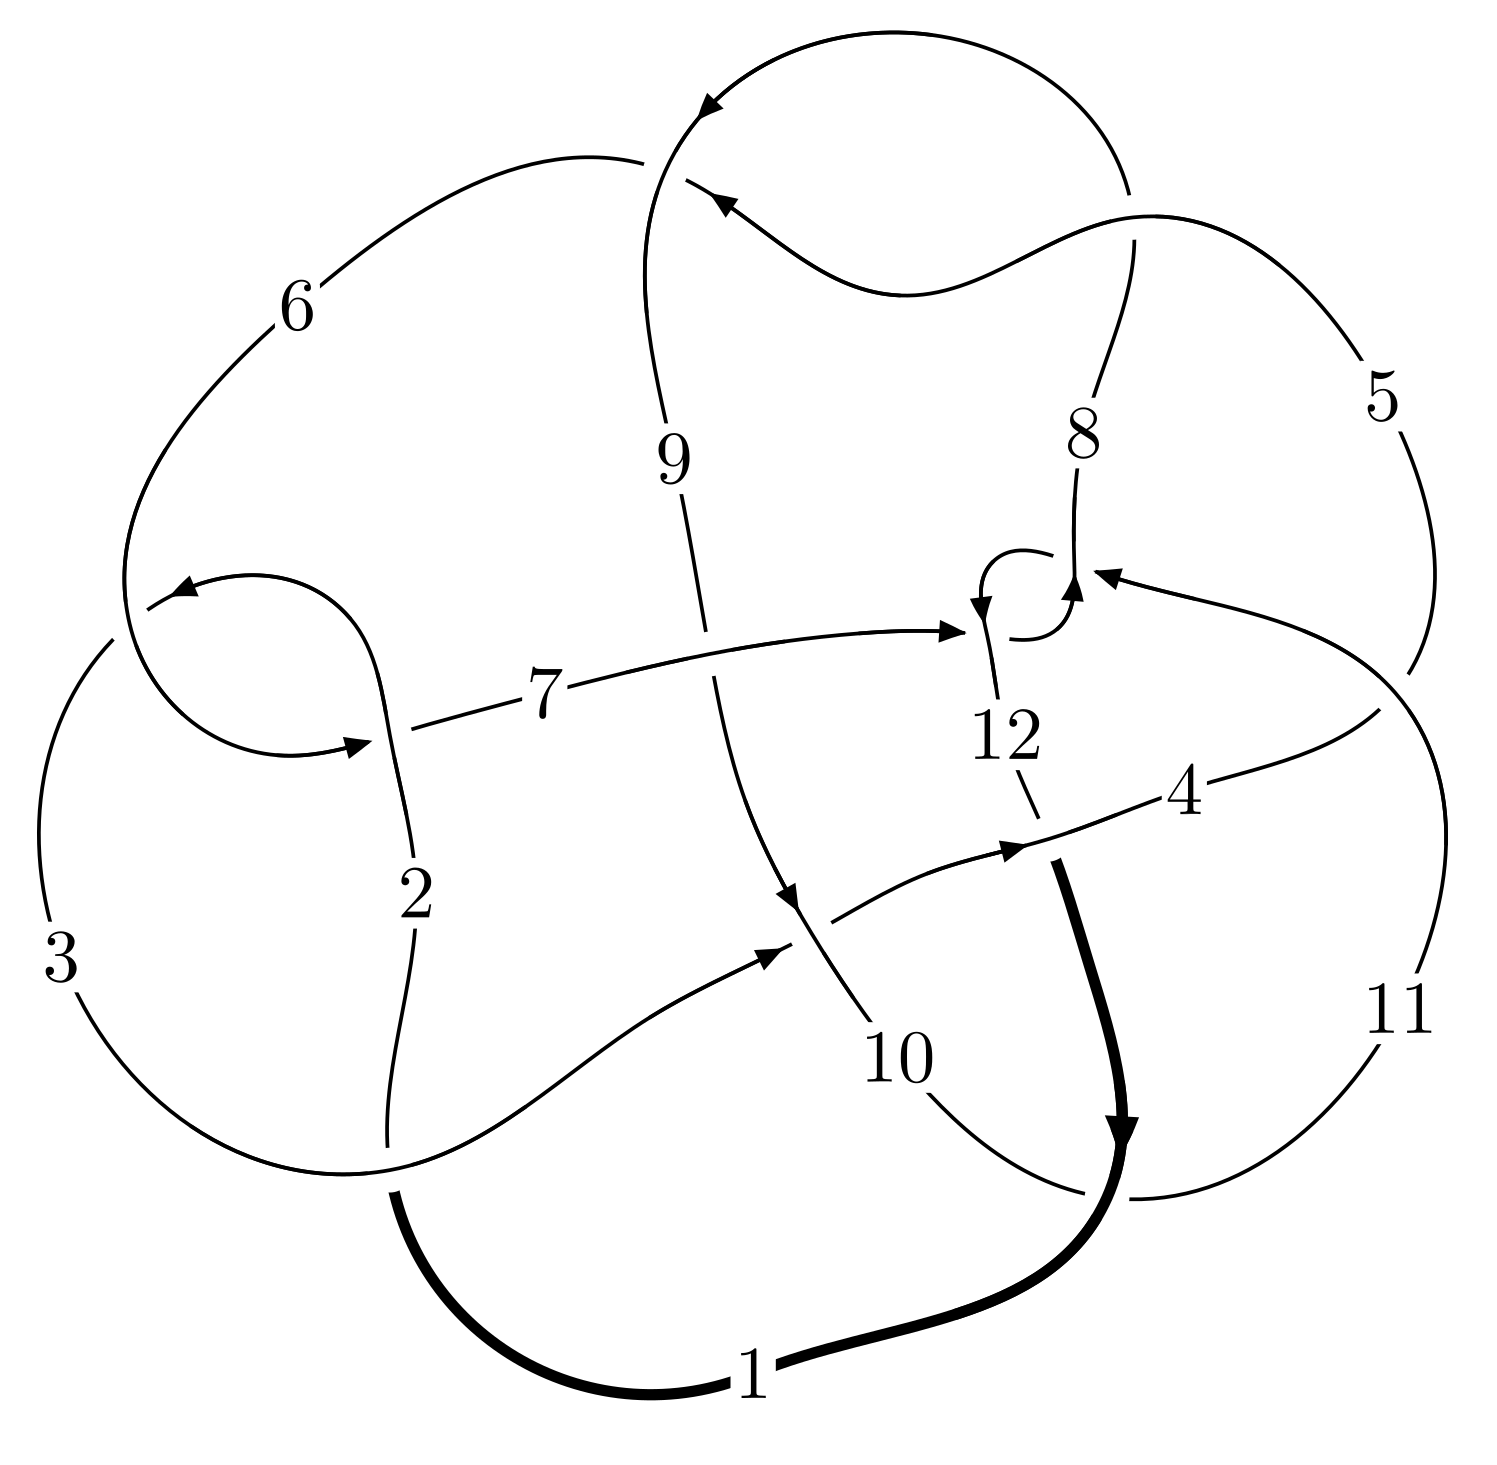
\includegraphics[width=112pt]{../../../GIT/diagram.site/Diagrams/png/1256_12a_0455.png}\\
\ \ \ A knot diagram\footnotemark}&
\allowdisplaybreaks
\textbf{Linearized knot diagam} \\
\cline{2-2}
 &
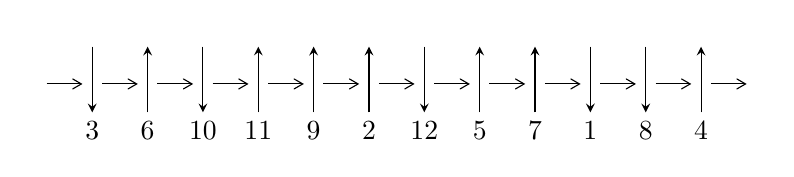
\begin{tikzpicture}[x=20pt, y=17pt]
	% nodes
	\node (C0) at (0, 0) {};
	\node (C1) at (1, 0) {};
	\node (C1U) at (1, +1) {};
	\node (C1D) at (1, -1) {3};

	\node (C2) at (2, 0) {};
	\node (C2U) at (2, +1) {};
	\node (C2D) at (2, -1) {6};

	\node (C3) at (3, 0) {};
	\node (C3U) at (3, +1) {};
	\node (C3D) at (3, -1) {10};

	\node (C4) at (4, 0) {};
	\node (C4U) at (4, +1) {};
	\node (C4D) at (4, -1) {11};

	\node (C5) at (5, 0) {};
	\node (C5U) at (5, +1) {};
	\node (C5D) at (5, -1) {9};

	\node (C6) at (6, 0) {};
	\node (C6U) at (6, +1) {};
	\node (C6D) at (6, -1) {2};

	\node (C7) at (7, 0) {};
	\node (C7U) at (7, +1) {};
	\node (C7D) at (7, -1) {12};

	\node (C8) at (8, 0) {};
	\node (C8U) at (8, +1) {};
	\node (C8D) at (8, -1) {5};

	\node (C9) at (9, 0) {};
	\node (C9U) at (9, +1) {};
	\node (C9D) at (9, -1) {7};

	\node (C10) at (10, 0) {};
	\node (C10U) at (10, +1) {};
	\node (C10D) at (10, -1) {1};

	\node (C11) at (11, 0) {};
	\node (C11U) at (11, +1) {};
	\node (C11D) at (11, -1) {8};

	\node (C12) at (12, 0) {};
	\node (C12U) at (12, +1) {};
	\node (C12D) at (12, -1) {4};
	\node (C13) at (13, 0) {};

	% arrows
	\draw[->,>={angle 60}]
	(C0) edge (C1) (C1) edge (C2) (C2) edge (C3) (C3) edge (C4) (C4) edge (C5) (C5) edge (C6) (C6) edge (C7) (C7) edge (C8) (C8) edge (C9) (C9) edge (C10) (C10) edge (C11) (C11) edge (C12) (C12) edge (C13) ;	\draw[->,>=stealth]
	(C1U) edge (C1D) (C2D) edge (C2U) (C3U) edge (C3D) (C4D) edge (C4U) (C5D) edge (C5U) (C6D) edge (C6U) (C7U) edge (C7D) (C8D) edge (C8U) (C9D) edge (C9U) (C10U) edge (C10D) (C11U) edge (C11D) (C12D) edge (C12U) ;
	\end{tikzpicture} \\
\hhline{~~} \\& 
\textbf{Solving Sequence} \\ \cline{2-2} 
 &
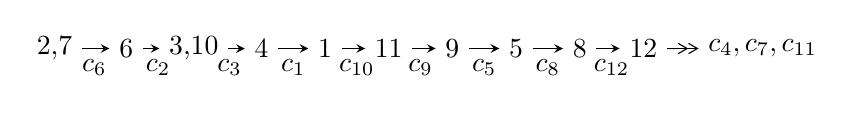
\begin{tikzpicture}[x=23pt, y=7pt]
	% node
	\node (A0) at (-1/8, 0) {2,7};
	\node (A1) at (1, 0) {6};
	\node (A2) at (33/16, 0) {3,10};
	\node (A3) at (25/8, 0) {4};
	\node (A4) at (33/8, 0) {1};
	\node (A5) at (41/8, 0) {11};
	\node (A6) at (49/8, 0) {9};
	\node (A7) at (57/8, 0) {5};
	\node (A8) at (65/8, 0) {8};
	\node (A9) at (73/8, 0) {12};
	\node (C1) at (1/2, -1) {$c_{6}$};
	\node (C2) at (3/2, -1) {$c_{2}$};
	\node (C3) at (21/8, -1) {$c_{3}$};
	\node (C4) at (29/8, -1) {$c_{1}$};
	\node (C5) at (37/8, -1) {$c_{10}$};
	\node (C6) at (45/8, -1) {$c_{9}$};
	\node (C7) at (53/8, -1) {$c_{5}$};
	\node (C8) at (61/8, -1) {$c_{8}$};
	\node (C9) at (69/8, -1) {$c_{12}$};
	\node (A10) at (11, 0) {$c_{4},c_{7},c_{11}$};

	% edge
	\draw[->,>=stealth]	
	(A0) edge (A1) (A1) edge (A2) (A2) edge (A3) (A3) edge (A4) (A4) edge (A5) (A5) edge (A6) (A6) edge (A7) (A7) edge (A8) (A8) edge (A9) ;
	\draw[->>,>={angle 60}]	
	(A9) edge (A10);
\end{tikzpicture} \\ 

\end{tabular} \\

\footnotetext{
The image of knot diagram is generated by the software ``\textbf{Draw programme}" developed by Andrew Bartholomew(\url{http://www.layer8.co.uk/maths/draw/index.htm\#Running-draw}), where we modified some parts for our purpose(\url{https://github.com/CATsTAILs/LinksPainter}).
}\phantom \\ \newline 
\centering \textbf{Ideals for irreducible components\footnotemark of $X_{\text{par}}$} 
 
\begin{align*}
I^u_{1}&=\langle 
-6.64159\times10^{351} u^{147}-2.04306\times10^{352} u^{146}+\cdots+3.22888\times10^{351} b-6.10666\times10^{352},\\
\phantom{I^u_{1}}&\phantom{= \langle  }-5.24126\times10^{351} u^{147}-1.21608\times10^{352} u^{146}+\cdots+3.22888\times10^{351} a+3.06698\times10^{353},\\
\phantom{I^u_{1}}&\phantom{= \langle  }u^{148}+2 u^{147}+\cdots+648 u-101\rangle \\
I^u_{2}&=\langle 
-98006 u^{28}-171495 u^{27}+\cdots+58439 b+136719,\\
\phantom{I^u_{2}}&\phantom{= \langle  }-178935 u^{28}-361858 u^{27}+\cdots+58439 a+408756,\;u^{29}+3 u^{28}+\cdots+2 u+1\rangle \\
\\
\end{align*}
\raggedright * 2 irreducible components of $\dim_{\mathbb{C}}=0$, with total 177 representations.\\
\footnotetext{All coefficients of polynomials are rational numbers. But the coefficients are sometimes approximated in decimal forms when there is not enough margin.}
\newpage
\renewcommand{\arraystretch}{1}
\centering \section*{I. $I^u_{1}= \langle -6.64\times10^{351} u^{147}-2.04\times10^{352} u^{146}+\cdots+3.23\times10^{351} b-6.11\times10^{352},\;-5.24\times10^{351} u^{147}-1.22\times10^{352} u^{146}+\cdots+3.23\times10^{351} a+3.07\times10^{353},\;u^{148}+2 u^{147}+\cdots+648 u-101 \rangle$}
\flushleft \textbf{(i) Arc colorings}\\
\begin{tabular}{m{7pt} m{180pt} m{7pt} m{180pt} }
\flushright $a_{2}=$&$\begin{pmatrix}0\\u\end{pmatrix}$ \\
\flushright $a_{7}=$&$\begin{pmatrix}1\\0\end{pmatrix}$ \\
\flushright $a_{6}=$&$\begin{pmatrix}1\\u^2\end{pmatrix}$ \\
\flushright $a_{3}=$&$\begin{pmatrix}u\\u^3+u\end{pmatrix}$ \\
\flushright $a_{10}=$&$\begin{pmatrix}1.62324 u^{147}+3.76624 u^{146}+\cdots+215.821 u-94.9857\\2.05693 u^{147}+6.32746 u^{146}+\cdots-394.089 u+18.9126\end{pmatrix}$ \\
\flushright $a_{4}=$&$\begin{pmatrix}-4.25834 u^{147}-13.7647 u^{146}+\cdots+536.061 u-8.91213\\-0.0989344 u^{147}-0.283071 u^{146}+\cdots-0.416518 u+1.70615\end{pmatrix}$ \\
\flushright $a_{1}=$&$\begin{pmatrix}u^3\\u^5+u^3+u\end{pmatrix}$ \\
\flushright $a_{11}=$&$\begin{pmatrix}0.340291 u^{147}-1.41193 u^{146}+\cdots+1.36267 u-28.3977\\0.935089 u^{147}+2.73408 u^{146}+\cdots-589.808 u+77.5672\end{pmatrix}$ \\
\flushright $a_{9}=$&$\begin{pmatrix}-0.433691 u^{147}-2.56122 u^{146}+\cdots+609.910 u-113.898\\2.05693 u^{147}+6.32746 u^{146}+\cdots-394.089 u+18.9126\end{pmatrix}$ \\
\flushright $a_{5}=$&$\begin{pmatrix}-4.15824 u^{147}-15.5606 u^{146}+\cdots-951.355 u+226.736\\-1.08619 u^{147}-1.41697 u^{146}+\cdots+1067.53 u-176.821\end{pmatrix}$ \\
\flushright $a_{8}=$&$\begin{pmatrix}14.5223 u^{147}+33.0084 u^{146}+\cdots-9219.44 u+1499.03\\-0.556047 u^{147}-2.33541 u^{146}+\cdots+46.6725 u+2.68327\end{pmatrix}$ \\
\flushright $a_{12}=$&$\begin{pmatrix}9.20435 u^{147}+43.3960 u^{146}+\cdots+7499.92 u-1579.10\\-0.0490474 u^{147}-0.557633 u^{146}+\cdots+138.617 u-22.2642\end{pmatrix}$\\&\end{tabular}
\flushleft \textbf{(ii) Obstruction class $= -1$}\\~\\
\flushleft \textbf{(iii) Cusp Shapes $= -23.7391 u^{147}-56.5982 u^{146}+\cdots+11427.9 u-1690.16$}\\~\\
\newpage\renewcommand{\arraystretch}{1}
\flushleft \textbf{(iv) u-Polynomials at the component}\newline \\
\begin{tabular}{m{50pt}|m{274pt}}
Crossings & \hspace{64pt}u-Polynomials at each crossing \\
\hline $$\begin{aligned}c_{1}\end{aligned}$$&$\begin{aligned}
&u^{148}+52 u^{147}+\cdots+225688 u+10201
\end{aligned}$\\
\hline $$\begin{aligned}c_{2},c_{6}\end{aligned}$$&$\begin{aligned}
&u^{148}+2 u^{147}+\cdots+648 u-101
\end{aligned}$\\
\hline $$\begin{aligned}c_{3}\end{aligned}$$&$\begin{aligned}
&u^{148}+6 u^{147}+\cdots-28 u+1
\end{aligned}$\\
\hline $$\begin{aligned}c_{4}\end{aligned}$$&$\begin{aligned}
&u^{148}- u^{147}+\cdots+58981664 u-6309529
\end{aligned}$\\
\hline $$\begin{aligned}c_{5},c_{8}\end{aligned}$$&$\begin{aligned}
&u^{148}+2 u^{147}+\cdots+569785 u+75377
\end{aligned}$\\
\hline $$\begin{aligned}c_{7},c_{11}\end{aligned}$$&$\begin{aligned}
&u^{148}- u^{147}+\cdots+20974 u-1021
\end{aligned}$\\
\hline $$\begin{aligned}c_{9}\end{aligned}$$&$\begin{aligned}
&u^{148}+17 u^{147}+\cdots+20173695 u+2908799
\end{aligned}$\\
\hline $$\begin{aligned}c_{10}\end{aligned}$$&$\begin{aligned}
&u^{148}-16 u^{147}+\cdots-121942 u+17011
\end{aligned}$\\
\hline $$\begin{aligned}c_{12}\end{aligned}$$&$\begin{aligned}
&u^{148}+3 u^{147}+\cdots-45 u-1
\end{aligned}$\\
\hline
\end{tabular}\\~\\
\newpage\renewcommand{\arraystretch}{1}
\flushleft \textbf{(v) Riley Polynomials at the component}\newline \\
\begin{tabular}{m{50pt}|m{274pt}}
Crossings & \hspace{64pt}Riley Polynomials at each crossing \\
\hline $$\begin{aligned}c_{1}\end{aligned}$$&$\begin{aligned}
&y^{148}+64 y^{147}+\cdots+1862038336 y+104060401
\end{aligned}$\\
\hline $$\begin{aligned}c_{2},c_{6}\end{aligned}$$&$\begin{aligned}
&y^{148}+52 y^{147}+\cdots+225688 y+10201
\end{aligned}$\\
\hline $$\begin{aligned}c_{3}\end{aligned}$$&$\begin{aligned}
&y^{148}+24 y^{147}+\cdots-116 y+1
\end{aligned}$\\
\hline $$\begin{aligned}c_{4}\end{aligned}$$&$\begin{aligned}
&y^{148}-59 y^{147}+\cdots-6005658867352188 y+39810156201841
\end{aligned}$\\
\hline $$\begin{aligned}c_{5},c_{8}\end{aligned}$$&$\begin{aligned}
&y^{148}-110 y^{147}+\cdots-159118159739 y+5681692129
\end{aligned}$\\
\hline $$\begin{aligned}c_{7},c_{11}\end{aligned}$$&$\begin{aligned}
&y^{148}+91 y^{147}+\cdots+140301120 y+1042441
\end{aligned}$\\
\hline $$\begin{aligned}c_{9}\end{aligned}$$&$\begin{aligned}
&y^{148}-57 y^{147}+\cdots-651689179521105 y+8461111622401
\end{aligned}$\\
\hline $$\begin{aligned}c_{10}\end{aligned}$$&$\begin{aligned}
&y^{148}+26 y^{147}+\cdots+23472466328 y+289374121
\end{aligned}$\\
\hline $$\begin{aligned}c_{12}\end{aligned}$$&$\begin{aligned}
&y^{148}-23 y^{147}+\cdots+47 y+1
\end{aligned}$\\
\hline
\end{tabular}\\~\\
\newpage\flushleft \textbf{(vi) Complex Volumes and Cusp Shapes}
$$\begin{array}{c|c|c}  
\text{Solutions to }I^u_{1}& \I (\text{vol} + \sqrt{-1}CS) & \text{Cusp shape}\\
 \hline 
\begin{aligned}
u &= -0.769936 + 0.637167 I \\
a &= \phantom{-}1.51306 + 1.57880 I \\
b &= \phantom{-}1.95693 + 0.78697 I\end{aligned}
 & \phantom{-}4.71739 + 4.12254 I & \phantom{-0.000000 } 0 \\ \hline\begin{aligned}
u &= -0.769936 - 0.637167 I \\
a &= \phantom{-}1.51306 - 1.57880 I \\
b &= \phantom{-}1.95693 - 0.78697 I\end{aligned}
 & \phantom{-}4.71739 - 4.12254 I & \phantom{-0.000000 } 0 \\ \hline\begin{aligned}
u &= \phantom{-}0.839915 + 0.558536 I \\
a &= -0.793268 - 0.504148 I \\
b &= -0.455550 - 0.818813 I\end{aligned}
 & \phantom{-}3.74720 + 4.69907 I & \phantom{-0.000000 } 0 \\ \hline\begin{aligned}
u &= \phantom{-}0.839915 - 0.558536 I \\
a &= -0.793268 + 0.504148 I \\
b &= -0.455550 + 0.818813 I\end{aligned}
 & \phantom{-}3.74720 - 4.69907 I & \phantom{-0.000000 } 0 \\ \hline\begin{aligned}
u &= \phantom{-}0.680603 + 0.758056 I \\
a &= -1.15384 + 1.70671 I \\
b &= -1.029920 + 0.371559 I\end{aligned}
 & \phantom{-}1.59469 - 1.18911 I & \phantom{-0.000000 } 0 \\ \hline\begin{aligned}
u &= \phantom{-}0.680603 - 0.758056 I \\
a &= -1.15384 - 1.70671 I \\
b &= -1.029920 - 0.371559 I\end{aligned}
 & \phantom{-}1.59469 + 1.18911 I & \phantom{-0.000000 } 0 \\ \hline\begin{aligned}
u &= \phantom{-}0.082421 + 0.975904 I \\
a &= \phantom{-}0.404354 + 0.748854 I \\
b &= -0.053861 - 1.256040 I\end{aligned}
 & -2.80448 + 2.17992 I & \phantom{-0.000000 } 0 \\ \hline\begin{aligned}
u &= \phantom{-}0.082421 - 0.975904 I \\
a &= \phantom{-}0.404354 - 0.748854 I \\
b &= -0.053861 + 1.256040 I\end{aligned}
 & -2.80448 - 2.17992 I & \phantom{-0.000000 } 0 \\ \hline\begin{aligned}
u &= -0.800073 + 0.642825 I \\
a &= -1.04329 - 1.29748 I \\
b &= -1.37614 - 0.90742 I\end{aligned}
 & \phantom{-}3.52532 + 2.68080 I & \phantom{-0.000000 } 0 \\ \hline\begin{aligned}
u &= -0.800073 - 0.642825 I \\
a &= -1.04329 + 1.29748 I \\
b &= -1.37614 + 0.90742 I\end{aligned}
 & \phantom{-}3.52532 - 2.68080 I & \phantom{-0.000000 } 0\\
 \hline 
 \end{array}$$\newpage$$\begin{array}{c|c|c}  
\text{Solutions to }I^u_{1}& \I (\text{vol} + \sqrt{-1}CS) & \text{Cusp shape}\\
 \hline 
\begin{aligned}
u &= \phantom{-}0.533509 + 0.810153 I \\
a &= -3.11459 + 2.72354 I \\
b &= -0.239845 - 0.209041 I\end{aligned}
 & \phantom{-}3.50091 + 1.82337 I & \phantom{-0.000000 } 0 \\ \hline\begin{aligned}
u &= \phantom{-}0.533509 - 0.810153 I \\
a &= -3.11459 - 2.72354 I \\
b &= -0.239845 + 0.209041 I\end{aligned}
 & \phantom{-}3.50091 - 1.82337 I & \phantom{-0.000000 } 0 \\ \hline\begin{aligned}
u &= -0.692022 + 0.774667 I \\
a &= \phantom{-}1.47729 + 0.28878 I \\
b &= \phantom{-}1.40281 + 0.46749 I\end{aligned}
 & \phantom{-}9.60483 + 5.04060 I & \phantom{-0.000000 } 0 \\ \hline\begin{aligned}
u &= -0.692022 - 0.774667 I \\
a &= \phantom{-}1.47729 - 0.28878 I \\
b &= \phantom{-}1.40281 - 0.46749 I\end{aligned}
 & \phantom{-}9.60483 - 5.04060 I & \phantom{-0.000000 } 0 \\ \hline\begin{aligned}
u &= -0.800256 + 0.519923 I \\
a &= -1.12012 - 0.88361 I \\
b &= -0.686300 - 0.823247 I\end{aligned}
 & \phantom{-}3.56002 + 8.07451 I & \phantom{-0.000000 } 0 \\ \hline\begin{aligned}
u &= -0.800256 - 0.519923 I \\
a &= -1.12012 + 0.88361 I \\
b &= -0.686300 + 0.823247 I\end{aligned}
 & \phantom{-}3.56002 - 8.07451 I & \phantom{-0.000000 } 0 \\ \hline\begin{aligned}
u &= \phantom{-}0.614932 + 0.846163 I \\
a &= -1.54915 + 1.00418 I \\
b &= -0.74713 - 1.28581 I\end{aligned}
 & \phantom{-}3.47362 + 0.56739 I & \phantom{-0.000000 } 0 \\ \hline\begin{aligned}
u &= \phantom{-}0.614932 - 0.846163 I \\
a &= -1.54915 - 1.00418 I \\
b &= -0.74713 + 1.28581 I\end{aligned}
 & \phantom{-}3.47362 - 0.56739 I & \phantom{-0.000000 } 0 \\ \hline\begin{aligned}
u &= \phantom{-}0.637209 + 0.831340 I \\
a &= \phantom{-}0.84150 - 2.10274 I \\
b &= \phantom{-}2.48068 - 1.44697 I\end{aligned}
 & \phantom{-}8.44146 + 7.98648 I & \phantom{-0.000000 } 0 \\ \hline\begin{aligned}
u &= \phantom{-}0.637209 - 0.831340 I \\
a &= \phantom{-}0.84150 + 2.10274 I \\
b &= \phantom{-}2.48068 + 1.44697 I\end{aligned}
 & \phantom{-}8.44146 - 7.98648 I & \phantom{-0.000000 } 0\\
 \hline 
 \end{array}$$\newpage$$\begin{array}{c|c|c}  
\text{Solutions to }I^u_{1}& \I (\text{vol} + \sqrt{-1}CS) & \text{Cusp shape}\\
 \hline 
\begin{aligned}
u &= -0.706571 + 0.785069 I \\
a &= -0.918845 - 0.481131 I \\
b &= -1.237320 - 0.660865 I\end{aligned}
 & \phantom{-}5.75577 + 0.28751 I & \phantom{-0.000000 } 0 \\ \hline\begin{aligned}
u &= -0.706571 - 0.785069 I \\
a &= -0.918845 + 0.481131 I \\
b &= -1.237320 + 0.660865 I\end{aligned}
 & \phantom{-}5.75577 - 0.28751 I & \phantom{-0.000000 } 0 \\ \hline\begin{aligned}
u &= \phantom{-}0.655402 + 0.678853 I \\
a &= \phantom{-}0.960142 - 0.391166 I \\
b &= \phantom{-}0.345528 + 0.044798 I\end{aligned}
 & \phantom{-}1.36746 + 1.48211 I & \phantom{-0.000000 } 0 \\ \hline\begin{aligned}
u &= \phantom{-}0.655402 - 0.678853 I \\
a &= \phantom{-}0.960142 + 0.391166 I \\
b &= \phantom{-}0.345528 - 0.044798 I\end{aligned}
 & \phantom{-}1.36746 - 1.48211 I & \phantom{-0.000000 } 0 \\ \hline\begin{aligned}
u &= \phantom{-}0.057886 + 1.055360 I \\
a &= -0.742576 - 0.161146 I \\
b &= \phantom{-}0.864498 + 1.006030 I\end{aligned}
 & -1.09038 + 3.64274 I & \phantom{-0.000000 } 0 \\ \hline\begin{aligned}
u &= \phantom{-}0.057886 - 1.055360 I \\
a &= -0.742576 + 0.161146 I \\
b &= \phantom{-}0.864498 - 1.006030 I\end{aligned}
 & -1.09038 - 3.64274 I & \phantom{-0.000000 } 0 \\ \hline\begin{aligned}
u &= \phantom{-}0.612091 + 0.863181 I \\
a &= -0.388473 + 0.671927 I \\
b &= -1.17312 + 1.22060 I\end{aligned}
 & \phantom{-}3.42037 + 4.25835 I & \phantom{-0.000000 } 0 \\ \hline\begin{aligned}
u &= \phantom{-}0.612091 - 0.863181 I \\
a &= -0.388473 - 0.671927 I \\
b &= -1.17312 - 1.22060 I\end{aligned}
 & \phantom{-}3.42037 - 4.25835 I & \phantom{-0.000000 } 0 \\ \hline\begin{aligned}
u &= -0.452159 + 0.957349 I \\
a &= \phantom{-}1.252100 + 0.655520 I \\
b &= \phantom{-}0.916740 - 0.482441 I\end{aligned}
 & -2.95953 - 1.60773 I & \phantom{-0.000000 } 0 \\ \hline\begin{aligned}
u &= -0.452159 - 0.957349 I \\
a &= \phantom{-}1.252100 - 0.655520 I \\
b &= \phantom{-}0.916740 + 0.482441 I\end{aligned}
 & -2.95953 + 1.60773 I & \phantom{-0.000000 } 0\\
 \hline 
 \end{array}$$\newpage$$\begin{array}{c|c|c}  
\text{Solutions to }I^u_{1}& \I (\text{vol} + \sqrt{-1}CS) & \text{Cusp shape}\\
 \hline 
\begin{aligned}
u &= -0.682346 + 0.645395 I \\
a &= -1.91385 - 0.70412 I \\
b &= -1.45467 + 0.53812 I\end{aligned}
 & \phantom{-}5.48460 + 1.98053 I & \phantom{-0.000000 } 0 \\ \hline\begin{aligned}
u &= -0.682346 - 0.645395 I \\
a &= -1.91385 + 0.70412 I \\
b &= -1.45467 - 0.53812 I\end{aligned}
 & \phantom{-}5.48460 - 1.98053 I & \phantom{-0.000000 } 0 \\ \hline\begin{aligned}
u &= \phantom{-}0.089356 + 1.057760 I \\
a &= \phantom{-}0.397022 + 0.533329 I \\
b &= -0.376259 - 1.046850 I\end{aligned}
 & -2.61567 + 2.29136 I & \phantom{-0.000000 } 0 \\ \hline\begin{aligned}
u &= \phantom{-}0.089356 - 1.057760 I \\
a &= \phantom{-}0.397022 - 0.533329 I \\
b &= -0.376259 + 1.046850 I\end{aligned}
 & -2.61567 - 2.29136 I & \phantom{-0.000000 } 0 \\ \hline\begin{aligned}
u &= \phantom{-}0.621686 + 0.698295 I \\
a &= \phantom{-}0.523634 - 1.135410 I \\
b &= \phantom{-}0.182883 - 0.355598 I\end{aligned}
 & \phantom{-}1.46921 + 1.77573 I & \phantom{-0.000000 } 0 \\ \hline\begin{aligned}
u &= \phantom{-}0.621686 - 0.698295 I \\
a &= \phantom{-}0.523634 + 1.135410 I \\
b &= \phantom{-}0.182883 + 0.355598 I\end{aligned}
 & \phantom{-}1.46921 - 1.77573 I & \phantom{-0.000000 } 0 \\ \hline\begin{aligned}
u &= -0.753687 + 0.758324 I \\
a &= \phantom{-}0.478102 - 0.190940 I \\
b &= \phantom{-}0.864382 + 0.396362 I\end{aligned}
 & \phantom{-}9.07722 - 4.51869 I & \phantom{-0.000000 } 0 \\ \hline\begin{aligned}
u &= -0.753687 - 0.758324 I \\
a &= \phantom{-}0.478102 + 0.190940 I \\
b &= \phantom{-}0.864382 - 0.396362 I\end{aligned}
 & \phantom{-}9.07722 + 4.51869 I & \phantom{-0.000000 } 0 \\ \hline\begin{aligned}
u &= -0.762931 + 0.524549 I \\
a &= \phantom{-}1.171310 + 0.733873 I \\
b &= \phantom{-}0.665422 + 0.379943 I\end{aligned}
 & \phantom{-}0.60685 + 3.89379 I & \phantom{-0.000000 } 0 \\ \hline\begin{aligned}
u &= -0.762931 - 0.524549 I \\
a &= \phantom{-}1.171310 - 0.733873 I \\
b &= \phantom{-}0.665422 - 0.379943 I\end{aligned}
 & \phantom{-}0.60685 - 3.89379 I & \phantom{-0.000000 } 0\\
 \hline 
 \end{array}$$\newpage$$\begin{array}{c|c|c}  
\text{Solutions to }I^u_{1}& \I (\text{vol} + \sqrt{-1}CS) & \text{Cusp shape}\\
 \hline 
\begin{aligned}
u &= \phantom{-}0.643856 + 0.877600 I \\
a &= \phantom{-}2.49371 - 1.18966 I \\
b &= \phantom{-}1.92963 + 1.77881 I\end{aligned}
 & \phantom{-}8.29501 - 2.98629 I & \phantom{-0.000000 } 0 \\ \hline\begin{aligned}
u &= \phantom{-}0.643856 - 0.877600 I \\
a &= \phantom{-}2.49371 + 1.18966 I \\
b &= \phantom{-}1.92963 - 1.77881 I\end{aligned}
 & \phantom{-}8.29501 + 2.98629 I & \phantom{-0.000000 } 0 \\ \hline\begin{aligned}
u &= \phantom{-}0.561460 + 0.933887 I \\
a &= -2.33444 + 0.83306 I \\
b &= -0.535764 - 0.033243 I\end{aligned}
 & \phantom{-}3.04732 + 2.54731 I & \phantom{-0.000000 } 0 \\ \hline\begin{aligned}
u &= \phantom{-}0.561460 - 0.933887 I \\
a &= -2.33444 - 0.83306 I \\
b &= -0.535764 + 0.033243 I\end{aligned}
 & \phantom{-}3.04732 - 2.54731 I & \phantom{-0.000000 } 0 \\ \hline\begin{aligned}
u &= \phantom{-}0.168089 + 1.076850 I \\
a &= -1.253420 - 0.599193 I \\
b &= \phantom{-}0.758942 - 1.037640 I\end{aligned}
 & \phantom{-}2.69789 - 3.74630 I & \phantom{-0.000000 } 0 \\ \hline\begin{aligned}
u &= \phantom{-}0.168089 - 1.076850 I \\
a &= -1.253420 + 0.599193 I \\
b &= \phantom{-}0.758942 + 1.037640 I\end{aligned}
 & \phantom{-}2.69789 + 3.74630 I & \phantom{-0.000000 } 0 \\ \hline\begin{aligned}
u &= \phantom{-}0.507455 + 0.983069 I \\
a &= \phantom{-}0.225480 - 1.144630 I \\
b &= \phantom{-}0.287681 + 0.146148 I\end{aligned}
 & \phantom{-}1.76820 + 2.11705 I & \phantom{-0.000000 } 0 \\ \hline\begin{aligned}
u &= \phantom{-}0.507455 - 0.983069 I \\
a &= \phantom{-}0.225480 + 1.144630 I \\
b &= \phantom{-}0.287681 - 0.146148 I\end{aligned}
 & \phantom{-}1.76820 - 2.11705 I & \phantom{-0.000000 } 0 \\ \hline\begin{aligned}
u &= \phantom{-}0.969721 + 0.534209 I \\
a &= \phantom{-}0.999737 - 0.607200 I \\
b &= \phantom{-}1.35067 - 0.42951 I\end{aligned}
 & \phantom{-}11.20750 - 1.13432 I & \phantom{-0.000000 } 0 \\ \hline\begin{aligned}
u &= \phantom{-}0.969721 - 0.534209 I \\
a &= \phantom{-}0.999737 + 0.607200 I \\
b &= \phantom{-}1.35067 + 0.42951 I\end{aligned}
 & \phantom{-}11.20750 + 1.13432 I & \phantom{-0.000000 } 0\\
 \hline 
 \end{array}$$\newpage$$\begin{array}{c|c|c}  
\text{Solutions to }I^u_{1}& \I (\text{vol} + \sqrt{-1}CS) & \text{Cusp shape}\\
 \hline 
\begin{aligned}
u &= -0.560989 + 0.958698 I \\
a &= -1.88637 - 0.49337 I \\
b &= -1.05468 + 1.18469 I\end{aligned}
 & \phantom{-}0.03616 - 6.60312 I & \phantom{-0.000000 } 0 \\ \hline\begin{aligned}
u &= -0.560989 - 0.958698 I \\
a &= -1.88637 + 0.49337 I \\
b &= -1.05468 - 1.18469 I\end{aligned}
 & \phantom{-}0.03616 + 6.60312 I & \phantom{-0.000000 } 0 \\ \hline\begin{aligned}
u &= -0.407500 + 1.035220 I \\
a &= -0.295263 + 0.385450 I \\
b &= \phantom{-}0.462997 + 1.110580 I\end{aligned}
 & -3.28286 - 4.45845 I & \phantom{-0.000000 } 0 \\ \hline\begin{aligned}
u &= -0.407500 - 1.035220 I \\
a &= -0.295263 - 0.385450 I \\
b &= \phantom{-}0.462997 - 1.110580 I\end{aligned}
 & -3.28286 + 4.45845 I & \phantom{-0.000000 } 0 \\ \hline\begin{aligned}
u &= \phantom{-}0.403619 + 0.789925 I \\
a &= \phantom{-}2.62780 + 1.73916 I \\
b &= \phantom{-}0.393620 - 0.088664 I\end{aligned}
 & \phantom{-}2.97332 + 1.73336 I & \phantom{-0.000000 } 0 \\ \hline\begin{aligned}
u &= \phantom{-}0.403619 - 0.789925 I \\
a &= \phantom{-}2.62780 - 1.73916 I \\
b &= \phantom{-}0.393620 + 0.088664 I\end{aligned}
 & \phantom{-}2.97332 - 1.73336 I & \phantom{-0.000000 } 0 \\ \hline\begin{aligned}
u &= \phantom{-}0.945252 + 0.591891 I \\
a &= \phantom{-}0.97609 - 1.12813 I \\
b &= \phantom{-}1.42305 - 1.01224 I\end{aligned}
 & \phantom{-}9.8462 - 13.8073 I & \phantom{-0.000000 } 0 \\ \hline\begin{aligned}
u &= \phantom{-}0.945252 - 0.591891 I \\
a &= \phantom{-}0.97609 + 1.12813 I \\
b &= \phantom{-}1.42305 + 1.01224 I\end{aligned}
 & \phantom{-}9.8462 + 13.8073 I & \phantom{-0.000000 } 0 \\ \hline\begin{aligned}
u &= -0.720337 + 0.855632 I \\
a &= \phantom{-}1.49256 - 0.38863 I \\
b &= \phantom{-}0.31089 - 1.94869 I\end{aligned}
 & \phantom{-}8.11074 - 2.09328 I & \phantom{-0.000000 } 0 \\ \hline\begin{aligned}
u &= -0.720337 - 0.855632 I \\
a &= \phantom{-}1.49256 + 0.38863 I \\
b &= \phantom{-}0.31089 + 1.94869 I\end{aligned}
 & \phantom{-}8.11074 + 2.09328 I & \phantom{-0.000000 } 0\\
 \hline 
 \end{array}$$\newpage$$\begin{array}{c|c|c}  
\text{Solutions to }I^u_{1}& \I (\text{vol} + \sqrt{-1}CS) & \text{Cusp shape}\\
 \hline 
\begin{aligned}
u &= -0.970205 + 0.562492 I \\
a &= \phantom{-}0.792995 + 0.503182 I \\
b &= \phantom{-}1.143020 + 0.679410 I\end{aligned}
 & \phantom{-}11.36020 + 4.55682 I & \phantom{-0.000000 } 0 \\ \hline\begin{aligned}
u &= -0.970205 - 0.562492 I \\
a &= \phantom{-}0.792995 - 0.503182 I \\
b &= \phantom{-}1.143020 - 0.679410 I\end{aligned}
 & \phantom{-}11.36020 - 4.55682 I & \phantom{-0.000000 } 0 \\ \hline\begin{aligned}
u &= -0.264987 + 0.833730 I \\
a &= \phantom{-}1.295610 + 0.229529 I \\
b &= -0.22044 - 1.42663 I\end{aligned}
 & -1.99613 + 1.72020 I & \phantom{-0.000000 } 0 \\ \hline\begin{aligned}
u &= -0.264987 - 0.833730 I \\
a &= \phantom{-}1.295610 - 0.229529 I \\
b &= -0.22044 + 1.42663 I\end{aligned}
 & -1.99613 - 1.72020 I & \phantom{-0.000000 } 0 \\ \hline\begin{aligned}
u &= -0.723000 + 0.862554 I \\
a &= -0.683099 + 1.095530 I \\
b &= \phantom{-}0.80358 + 1.86055 I\end{aligned}
 & \phantom{-}8.09150 - 3.40596 I & \phantom{-0.000000 } 0 \\ \hline\begin{aligned}
u &= -0.723000 - 0.862554 I \\
a &= -0.683099 - 1.095530 I \\
b &= \phantom{-}0.80358 - 1.86055 I\end{aligned}
 & \phantom{-}8.09150 + 3.40596 I & \phantom{-0.000000 } 0 \\ \hline\begin{aligned}
u &= \phantom{-}0.974867 + 0.589626 I \\
a &= -0.843848 + 0.942740 I \\
b &= -1.25978 + 0.82521 I\end{aligned}
 & \phantom{-}5.65662 - 7.35879 I & \phantom{-0.000000 } 0 \\ \hline\begin{aligned}
u &= \phantom{-}0.974867 - 0.589626 I \\
a &= -0.843848 - 0.942740 I \\
b &= -1.25978 - 0.82521 I\end{aligned}
 & \phantom{-}5.65662 + 7.35879 I & \phantom{-0.000000 } 0 \\ \hline\begin{aligned}
u &= -0.684381 + 0.913268 I \\
a &= -1.37694 - 1.09207 I \\
b &= -0.944280 + 0.860168 I\end{aligned}
 & \phantom{-}5.36543 - 5.62427 I & \phantom{-0.000000 } 0 \\ \hline\begin{aligned}
u &= -0.684381 - 0.913268 I \\
a &= -1.37694 + 1.09207 I \\
b &= -0.944280 - 0.860168 I\end{aligned}
 & \phantom{-}5.36543 + 5.62427 I & \phantom{-0.000000 } 0\\
 \hline 
 \end{array}$$\newpage$$\begin{array}{c|c|c}  
\text{Solutions to }I^u_{1}& \I (\text{vol} + \sqrt{-1}CS) & \text{Cusp shape}\\
 \hline 
\begin{aligned}
u &= -0.673284 + 0.923035 I \\
a &= \phantom{-}1.39343 + 1.65016 I \\
b &= \phantom{-}1.121090 - 0.595959 I\end{aligned}
 & \phantom{-}9.15061 - 10.30330 I & \phantom{-0.000000 } 0 \\ \hline\begin{aligned}
u &= -0.673284 - 0.923035 I \\
a &= \phantom{-}1.39343 - 1.65016 I \\
b &= \phantom{-}1.121090 + 0.595959 I\end{aligned}
 & \phantom{-}9.15061 + 10.30330 I & \phantom{-0.000000 } 0 \\ \hline\begin{aligned}
u &= \phantom{-}0.662223 + 0.937029 I \\
a &= -2.03763 + 0.25010 I \\
b &= -1.29671 - 0.67584 I\end{aligned}
 & \phantom{-}1.04599 + 6.38778 I & \phantom{-0.000000 } 0 \\ \hline\begin{aligned}
u &= \phantom{-}0.662223 - 0.937029 I \\
a &= -2.03763 - 0.25010 I \\
b &= -1.29671 + 0.67584 I\end{aligned}
 & \phantom{-}1.04599 - 6.38778 I & \phantom{-0.000000 } 0 \\ \hline\begin{aligned}
u &= -0.012214 + 1.151280 I \\
a &= \phantom{-}0.218582 - 0.257400 I \\
b &= \phantom{-}0.254769 + 0.881110 I\end{aligned}
 & -5.03626 + 2.30131 I & \phantom{-0.000000 } 0 \\ \hline\begin{aligned}
u &= -0.012214 - 1.151280 I \\
a &= \phantom{-}0.218582 + 0.257400 I \\
b &= \phantom{-}0.254769 - 0.881110 I\end{aligned}
 & -5.03626 - 2.30131 I & \phantom{-0.000000 } 0 \\ \hline\begin{aligned}
u &= \phantom{-}0.104267 + 0.841355 I \\
a &= -0.140788 - 0.834366 I \\
b &= -0.66639 + 1.35029 I\end{aligned}
 & -2.32899 - 2.11126 I & \phantom{-0.000000 } 0 \\ \hline\begin{aligned}
u &= \phantom{-}0.104267 - 0.841355 I \\
a &= -0.140788 + 0.834366 I \\
b &= -0.66639 - 1.35029 I\end{aligned}
 & -2.32899 + 2.11126 I & \phantom{-0.000000 } 0 \\ \hline\begin{aligned}
u &= -1.110010 + 0.319340 I \\
a &= \phantom{-}0.332488 - 0.230503 I \\
b &= \phantom{-}0.763772 - 0.118071 I\end{aligned}
 & \phantom{-}8.09797 - 8.18527 I & \phantom{-0.000000 } 0 \\ \hline\begin{aligned}
u &= -1.110010 - 0.319340 I \\
a &= \phantom{-}0.332488 + 0.230503 I \\
b &= \phantom{-}0.763772 + 0.118071 I\end{aligned}
 & \phantom{-}8.09797 + 8.18527 I & \phantom{-0.000000 } 0\\
 \hline 
 \end{array}$$\newpage$$\begin{array}{c|c|c}  
\text{Solutions to }I^u_{1}& \I (\text{vol} + \sqrt{-1}CS) & \text{Cusp shape}\\
 \hline 
\begin{aligned}
u &= \phantom{-}0.624567 + 0.980093 I \\
a &= \phantom{-}1.216560 - 0.241582 I \\
b &= \phantom{-}0.589137 + 0.338322 I\end{aligned}
 & \phantom{-}0.45205 + 3.50465 I & \phantom{-0.000000 } 0 \\ \hline\begin{aligned}
u &= \phantom{-}0.624567 - 0.980093 I \\
a &= \phantom{-}1.216560 + 0.241582 I \\
b &= \phantom{-}0.589137 - 0.338322 I\end{aligned}
 & \phantom{-}0.45205 - 3.50465 I & \phantom{-0.000000 } 0 \\ \hline\begin{aligned}
u &= \phantom{-}0.641338 + 0.975824 I \\
a &= \phantom{-}1.53440 + 0.25176 I \\
b &= \phantom{-}0.533710 + 0.685958 I\end{aligned}
 & \phantom{-}0.60913 + 3.24526 I & \phantom{-0.000000 } 0 \\ \hline\begin{aligned}
u &= \phantom{-}0.641338 - 0.975824 I \\
a &= \phantom{-}1.53440 - 0.25176 I \\
b &= \phantom{-}0.533710 - 0.685958 I\end{aligned}
 & \phantom{-}0.60913 - 3.24526 I & \phantom{-0.000000 } 0 \\ \hline\begin{aligned}
u &= \phantom{-}0.004974 + 1.167720 I \\
a &= -0.080516 + 0.577376 I \\
b &= -0.466323 - 1.085310 I\end{aligned}
 & -2.35243 + 6.40725 I & \phantom{-0.000000 } 0 \\ \hline\begin{aligned}
u &= \phantom{-}0.004974 - 1.167720 I \\
a &= -0.080516 - 0.577376 I \\
b &= -0.466323 + 1.085310 I\end{aligned}
 & -2.35243 - 6.40725 I & \phantom{-0.000000 } 0 \\ \hline\begin{aligned}
u &= -0.636773 + 0.997265 I \\
a &= -1.00898 - 1.26124 I \\
b &= -1.70064 - 0.15421 I\end{aligned}
 & \phantom{-}4.42882 - 7.10812 I & \phantom{-0.000000 } 0 \\ \hline\begin{aligned}
u &= -0.636773 - 0.997265 I \\
a &= -1.00898 + 1.26124 I \\
b &= -1.70064 + 0.15421 I\end{aligned}
 & \phantom{-}4.42882 + 7.10812 I & \phantom{-0.000000 } 0 \\ \hline\begin{aligned}
u &= \phantom{-}0.593681 + 1.023540 I \\
a &= \phantom{-}1.91308 - 1.26775 I \\
b &= \phantom{-}2.02863 + 1.49595 I\end{aligned}
 & \phantom{-}5.35359 + 10.26120 I & \phantom{-0.000000 } 0 \\ \hline\begin{aligned}
u &= \phantom{-}0.593681 - 1.023540 I \\
a &= \phantom{-}1.91308 + 1.26775 I \\
b &= \phantom{-}2.02863 - 1.49595 I\end{aligned}
 & \phantom{-}5.35359 - 10.26120 I & \phantom{-0.000000 } 0\\
 \hline 
 \end{array}$$\newpage$$\begin{array}{c|c|c}  
\text{Solutions to }I^u_{1}& \I (\text{vol} + \sqrt{-1}CS) & \text{Cusp shape}\\
 \hline 
\begin{aligned}
u &= -0.726251 + 0.939284 I \\
a &= \phantom{-}0.470063 + 0.833587 I \\
b &= \phantom{-}0.401942 - 0.566172 I\end{aligned}
 & \phantom{-}8.54049 - 1.08703 I & \phantom{-0.000000 } 0 \\ \hline\begin{aligned}
u &= -0.726251 - 0.939284 I \\
a &= \phantom{-}0.470063 - 0.833587 I \\
b &= \phantom{-}0.401942 + 0.566172 I\end{aligned}
 & \phantom{-}8.54049 + 1.08703 I & \phantom{-0.000000 } 0 \\ \hline\begin{aligned}
u &= \phantom{-}0.784216 + 0.208011 I \\
a &= -0.436489 - 0.104406 I \\
b &= -0.675779 - 0.006893 I\end{aligned}
 & \phantom{-}1.49213 + 0.09418 I & \phantom{-0.000000 } 0 \\ \hline\begin{aligned}
u &= \phantom{-}0.784216 - 0.208011 I \\
a &= -0.436489 + 0.104406 I \\
b &= -0.675779 + 0.006893 I\end{aligned}
 & \phantom{-}1.49213 - 0.09418 I & \phantom{-0.000000 } 0 \\ \hline\begin{aligned}
u &= \phantom{-}0.040675 + 0.789751 I \\
a &= -2.37348 - 0.75443 I \\
b &= \phantom{-}0.843461 - 0.529432 I\end{aligned}
 & \phantom{-}5.30954 + 6.50829 I & \phantom{-0.000000 } 0 \\ \hline\begin{aligned}
u &= \phantom{-}0.040675 - 0.789751 I \\
a &= -2.37348 + 0.75443 I \\
b &= \phantom{-}0.843461 + 0.529432 I\end{aligned}
 & \phantom{-}5.30954 - 6.50829 I & \phantom{-0.000000 } 0 \\ \hline\begin{aligned}
u &= \phantom{-}0.305796 + 0.708854 I \\
a &= -1.71675 + 0.18701 I \\
b &= -1.324070 - 0.241356 I\end{aligned}
 & \phantom{-}1.62553 - 0.93392 I & \phantom{-0.000000 } 0 \\ \hline\begin{aligned}
u &= \phantom{-}0.305796 - 0.708854 I \\
a &= -1.71675 - 0.18701 I \\
b &= -1.324070 + 0.241356 I\end{aligned}
 & \phantom{-}1.62553 + 0.93392 I & \phantom{-0.000000 } 0 \\ \hline\begin{aligned}
u &= -0.685085 + 1.020030 I \\
a &= \phantom{-}2.13374 + 1.10489 I \\
b &= \phantom{-}2.01427 - 1.25903 I\end{aligned}
 & \phantom{-}3.57308 - 9.64410 I & \phantom{-0.000000 } 0 \\ \hline\begin{aligned}
u &= -0.685085 - 1.020030 I \\
a &= \phantom{-}2.13374 - 1.10489 I \\
b &= \phantom{-}2.01427 + 1.25903 I\end{aligned}
 & \phantom{-}3.57308 + 9.64410 I & \phantom{-0.000000 } 0\\
 \hline 
 \end{array}$$\newpage$$\begin{array}{c|c|c}  
\text{Solutions to }I^u_{1}& \I (\text{vol} + \sqrt{-1}CS) & \text{Cusp shape}\\
 \hline 
\begin{aligned}
u &= \phantom{-}0.442510 + 1.149600 I \\
a &= -0.026493 + 1.316140 I \\
b &= -1.42405 + 0.27976 I\end{aligned}
 & -0.93725 + 4.03007 I & \phantom{-0.000000 } 0 \\ \hline\begin{aligned}
u &= \phantom{-}0.442510 - 1.149600 I \\
a &= -0.026493 - 1.316140 I \\
b &= -1.42405 - 0.27976 I\end{aligned}
 & -0.93725 - 4.03007 I & \phantom{-0.000000 } 0 \\ \hline\begin{aligned}
u &= -0.651514 + 1.055880 I \\
a &= \phantom{-}1.45529 + 0.49378 I \\
b &= \phantom{-}0.942923 - 0.567650 I\end{aligned}
 & -0.93890 - 9.25981 I & \phantom{-0.000000 } 0 \\ \hline\begin{aligned}
u &= -0.651514 - 1.055880 I \\
a &= \phantom{-}1.45529 - 0.49378 I \\
b &= \phantom{-}0.942923 + 0.567650 I\end{aligned}
 & -0.93890 + 9.25981 I & \phantom{-0.000000 } 0 \\ \hline\begin{aligned}
u &= -0.697643 + 1.026390 I \\
a &= -1.95036 - 0.65491 I \\
b &= -1.43148 + 1.28621 I\end{aligned}
 & \phantom{-}2.36887 - 8.32288 I & \phantom{-0.000000 } 0 \\ \hline\begin{aligned}
u &= -0.697643 - 1.026390 I \\
a &= -1.95036 + 0.65491 I \\
b &= -1.43148 - 1.28621 I\end{aligned}
 & \phantom{-}2.36887 + 8.32288 I & \phantom{-0.000000 } 0 \\ \hline\begin{aligned}
u &= \phantom{-}0.494245 + 0.566912 I \\
a &= \phantom{-}1.46375 - 1.82890 I \\
b &= \phantom{-}2.19364 - 0.56420 I\end{aligned}
 & \phantom{-}6.73797 - 5.59726 I & \phantom{-0.000000 } 0 \\ \hline\begin{aligned}
u &= \phantom{-}0.494245 - 0.566912 I \\
a &= \phantom{-}1.46375 + 1.82890 I \\
b &= \phantom{-}2.19364 + 0.56420 I\end{aligned}
 & \phantom{-}6.73797 + 5.59726 I & \phantom{-0.000000 } 0 \\ \hline\begin{aligned}
u &= \phantom{-}0.618970 + 1.090940 I \\
a &= -0.898525 + 0.614785 I \\
b &= -0.872745 - 0.708459 I\end{aligned}
 & -0.82047 + 5.13370 I & \phantom{-0.000000 } 0 \\ \hline\begin{aligned}
u &= \phantom{-}0.618970 - 1.090940 I \\
a &= -0.898525 - 0.614785 I \\
b &= -0.872745 + 0.708459 I\end{aligned}
 & -0.82047 - 5.13370 I & \phantom{-0.000000 } 0\\
 \hline 
 \end{array}$$\newpage$$\begin{array}{c|c|c}  
\text{Solutions to }I^u_{1}& \I (\text{vol} + \sqrt{-1}CS) & \text{Cusp shape}\\
 \hline 
\begin{aligned}
u &= -0.658937 + 1.067600 I \\
a &= -1.77396 - 0.49014 I \\
b &= -0.876392 + 0.917845 I\end{aligned}
 & \phantom{-}1.94680 - 13.55350 I & \phantom{-0.000000 } 0 \\ \hline\begin{aligned}
u &= -0.658937 - 1.067600 I \\
a &= -1.77396 + 0.49014 I \\
b &= -0.876392 - 0.917845 I\end{aligned}
 & \phantom{-}1.94680 + 13.55350 I & \phantom{-0.000000 } 0 \\ \hline\begin{aligned}
u &= -0.446704 + 0.586220 I \\
a &= -0.48099 - 1.47582 I \\
b &= -0.802919 - 0.715224 I\end{aligned}
 & \phantom{-}1.04584 + 2.26494 I & \phantom{-0.000000 } 0 \\ \hline\begin{aligned}
u &= -0.446704 - 0.586220 I \\
a &= -0.48099 + 1.47582 I \\
b &= -0.802919 + 0.715224 I\end{aligned}
 & \phantom{-}1.04584 - 2.26494 I & \phantom{-0.000000 } 0 \\ \hline\begin{aligned}
u &= -0.161935 + 1.269120 I \\
a &= -0.325955 + 0.253893 I \\
b &= \phantom{-}0.692576 - 0.850020 I\end{aligned}
 & \phantom{-}2.24682 - 12.10360 I & \phantom{-0.000000 } 0 \\ \hline\begin{aligned}
u &= -0.161935 - 1.269120 I \\
a &= -0.325955 - 0.253893 I \\
b &= \phantom{-}0.692576 + 0.850020 I\end{aligned}
 & \phantom{-}2.24682 + 12.10360 I & \phantom{-0.000000 } 0 \\ \hline\begin{aligned}
u &= \phantom{-}0.002432 + 0.719130 I \\
a &= \phantom{-}0.054436 - 1.142880 I \\
b &= -0.659458 - 0.250629 I\end{aligned}
 & \phantom{-}1.09994 + 2.09658 I & \phantom{-0.000000 } 0 \\ \hline\begin{aligned}
u &= \phantom{-}0.002432 - 0.719130 I \\
a &= \phantom{-}0.054436 + 1.142880 I \\
b &= -0.659458 + 0.250629 I\end{aligned}
 & \phantom{-}1.09994 - 2.09658 I & \phantom{-0.000000 } 0 \\ \hline\begin{aligned}
u &= \phantom{-}0.116144 + 0.674757 I \\
a &= \phantom{-}2.25606 + 0.81942 I \\
b &= -0.303519 + 0.183390 I\end{aligned}
 & \phantom{-}1.32804 + 2.45147 I & \phantom{-0.000000 } 0 \\ \hline\begin{aligned}
u &= \phantom{-}0.116144 - 0.674757 I \\
a &= \phantom{-}2.25606 - 0.81942 I \\
b &= -0.303519 - 0.183390 I\end{aligned}
 & \phantom{-}1.32804 - 2.45147 I & \phantom{-0.000000 } 0\\
 \hline 
 \end{array}$$\newpage$$\begin{array}{c|c|c}  
\text{Solutions to }I^u_{1}& \I (\text{vol} + \sqrt{-1}CS) & \text{Cusp shape}\\
 \hline 
\begin{aligned}
u &= \phantom{-}0.731434 + 1.102020 I \\
a &= \phantom{-}1.72781 - 0.69373 I \\
b &= \phantom{-}1.45412 + 1.29347 I\end{aligned}
 & \phantom{-}8.2610 + 19.9510 I & \phantom{-0.000000 } 0 \\ \hline\begin{aligned}
u &= \phantom{-}0.731434 - 1.102020 I \\
a &= \phantom{-}1.72781 + 0.69373 I \\
b &= \phantom{-}1.45412 - 1.29347 I\end{aligned}
 & \phantom{-}8.2610 - 19.9510 I & \phantom{-0.000000 } 0 \\ \hline\begin{aligned}
u &= -0.732177 + 1.115030 I \\
a &= \phantom{-}1.23441 + 0.75038 I \\
b &= \phantom{-}1.07674 - 0.97037 I\end{aligned}
 & \phantom{-}9.6528 - 10.7542 I & \phantom{-0.000000 } 0 \\ \hline\begin{aligned}
u &= -0.732177 - 1.115030 I \\
a &= \phantom{-}1.23441 - 0.75038 I \\
b &= \phantom{-}1.07674 + 0.97037 I\end{aligned}
 & \phantom{-}9.6528 + 10.7542 I & \phantom{-0.000000 } 0 \\ \hline\begin{aligned}
u &= -0.814338 + 1.056680 I \\
a &= -1.195400 - 0.029383 I \\
b &= -0.678119 + 1.217090 I\end{aligned}
 & \phantom{-}3.47314 - 6.90476 I & \phantom{-0.000000 } 0 \\ \hline\begin{aligned}
u &= -0.814338 - 1.056680 I \\
a &= -1.195400 + 0.029383 I \\
b &= -0.678119 - 1.217090 I\end{aligned}
 & \phantom{-}3.47314 + 6.90476 I & \phantom{-0.000000 } 0 \\ \hline\begin{aligned}
u &= \phantom{-}0.664233\phantom{ +0.000000I} \\
a &= -1.43464\phantom{ +0.000000I} \\
b &= -1.30578\phantom{ +0.000000I}\end{aligned}
 & \phantom{-}2.21894\phantom{ +0.000000I} & \phantom{-0.000000 } 0 \\ \hline\begin{aligned}
u &= \phantom{-}0.740118 + 1.112690 I \\
a &= -1.48718 + 0.59400 I \\
b &= -1.31169 - 1.11971 I\end{aligned}
 & \phantom{-}4.0208 + 13.6093 I & \phantom{-0.000000 } 0 \\ \hline\begin{aligned}
u &= \phantom{-}0.740118 - 1.112690 I \\
a &= -1.48718 - 0.59400 I \\
b &= -1.31169 + 1.11971 I\end{aligned}
 & \phantom{-}4.0208 - 13.6093 I & \phantom{-0.000000 } 0 \\ \hline\begin{aligned}
u &= \phantom{-}0.558940 + 0.357046 I \\
a &= \phantom{-}0.679118 + 1.146890 I \\
b &= \phantom{-}0.881939 + 0.002976 I\end{aligned}
 & \phantom{-}3.29262 + 2.11226 I & \phantom{-0.000000 } 0\\
 \hline 
 \end{array}$$\newpage$$\begin{array}{c|c|c}  
\text{Solutions to }I^u_{1}& \I (\text{vol} + \sqrt{-1}CS) & \text{Cusp shape}\\
 \hline 
\begin{aligned}
u &= \phantom{-}0.558940 - 0.357046 I \\
a &= \phantom{-}0.679118 - 1.146890 I \\
b &= \phantom{-}0.881939 - 0.002976 I\end{aligned}
 & \phantom{-}3.29262 - 2.11226 I & \phantom{-0.000000 } 0 \\ \hline\begin{aligned}
u &= \phantom{-}0.718741 + 1.129580 I \\
a &= \phantom{-}1.15158 - 0.82914 I \\
b &= \phantom{-}1.40120 + 0.75630 I\end{aligned}
 & \phantom{-}9.36834 + 7.28517 I & \phantom{-0.000000 } 0 \\ \hline\begin{aligned}
u &= \phantom{-}0.718741 - 1.129580 I \\
a &= \phantom{-}1.15158 + 0.82914 I \\
b &= \phantom{-}1.40120 - 0.75630 I\end{aligned}
 & \phantom{-}9.36834 - 7.28517 I & \phantom{-0.000000 } 0 \\ \hline\begin{aligned}
u &= \phantom{-}0.770563 + 1.099490 I \\
a &= \phantom{-}0.154330 + 0.226927 I \\
b &= -0.288914 + 0.455273 I\end{aligned}
 & \phantom{-}2.21026 + 1.19199 I & \phantom{-0.000000 } 0 \\ \hline\begin{aligned}
u &= \phantom{-}0.770563 - 1.099490 I \\
a &= \phantom{-}0.154330 - 0.226927 I \\
b &= -0.288914 - 0.455273 I\end{aligned}
 & \phantom{-}2.21026 - 1.19199 I & \phantom{-0.000000 } 0 \\ \hline\begin{aligned}
u &= -0.212852 + 1.326520 I \\
a &= \phantom{-}0.256717 - 0.093685 I \\
b &= -0.438676 + 0.606345 I\end{aligned}
 & -2.37008 - 5.40558 I & \phantom{-0.000000 } 0 \\ \hline\begin{aligned}
u &= -0.212852 - 1.326520 I \\
a &= \phantom{-}0.256717 + 0.093685 I \\
b &= -0.438676 - 0.606345 I\end{aligned}
 & -2.37008 + 5.40558 I & \phantom{-0.000000 } 0 \\ \hline\begin{aligned}
u &= -1.10012 + 0.89232 I \\
a &= \phantom{-}0.130966 - 0.447808 I \\
b &= -0.310512 - 0.812334 I\end{aligned}
 & \phantom{-}4.37587 + 0.05789 I & \phantom{-0.000000 } 0 \\ \hline\begin{aligned}
u &= -1.10012 - 0.89232 I \\
a &= \phantom{-}0.130966 + 0.447808 I \\
b &= -0.310512 + 0.812334 I\end{aligned}
 & \phantom{-}4.37587 - 0.05789 I & \phantom{-0.000000 } 0 \\ \hline\begin{aligned}
u &= -0.14302 + 1.45762 I \\
a &= -0.291389 - 0.025003 I \\
b &= \phantom{-}0.484017 - 0.114924 I\end{aligned}
 & \phantom{-}3.62994 + 1.54287 I & \phantom{-0.000000 } 0\\
 \hline 
 \end{array}$$\newpage$$\begin{array}{c|c|c}  
\text{Solutions to }I^u_{1}& \I (\text{vol} + \sqrt{-1}CS) & \text{Cusp shape}\\
 \hline 
\begin{aligned}
u &= -0.14302 - 1.45762 I \\
a &= -0.291389 + 0.025003 I \\
b &= \phantom{-}0.484017 + 0.114924 I\end{aligned}
 & \phantom{-}3.62994 - 1.54287 I & \phantom{-0.000000 } 0 \\ \hline\begin{aligned}
u &= \phantom{-}0.353163 + 0.317005 I \\
a &= \phantom{-}1.76206 - 1.80707 I \\
b &= \phantom{-}1.77187 - 0.30182 I\end{aligned}
 & \phantom{-}6.70775 - 5.64468 I & \phantom{-}2.91883 + 3.12758 I \\ \hline\begin{aligned}
u &= \phantom{-}0.353163 - 0.317005 I \\
a &= \phantom{-}1.76206 + 1.80707 I \\
b &= \phantom{-}1.77187 + 0.30182 I\end{aligned}
 & \phantom{-}6.70775 + 5.64468 I & \phantom{-}2.91883 - 3.12758 I \\ \hline\begin{aligned}
u &= \phantom{-}0.400843 + 0.239268 I \\
a &= -1.18485 - 1.81069 I \\
b &= -0.467740 + 0.579961 I\end{aligned}
 & \phantom{-}4.06649 + 1.04747 I & \phantom{-}8.01975 + 0.93073 I \\ \hline\begin{aligned}
u &= \phantom{-}0.400843 - 0.239268 I \\
a &= -1.18485 + 1.81069 I \\
b &= -0.467740 - 0.579961 I\end{aligned}
 & \phantom{-}4.06649 - 1.04747 I & \phantom{-}8.01975 - 0.93073 I \\ \hline\begin{aligned}
u &= -0.410832 + 0.000981 I \\
a &= \phantom{-}1.21699 - 1.41861 I \\
b &= \phantom{-}0.131418 - 0.538352 I\end{aligned}
 & -0.92136 + 1.37626 I & -1.95062 - 4.54782 I \\ \hline\begin{aligned}
u &= -0.410832 - 0.000981 I \\
a &= \phantom{-}1.21699 + 1.41861 I \\
b &= \phantom{-}0.131418 + 0.538352 I\end{aligned}
 & -0.92136 - 1.37626 I & -1.95062 + 4.54782 I \\ \hline\begin{aligned}
u &= -2.03244\phantom{ +0.000000I} \\
a &= -0.0421868\phantom{ +0.000000I} \\
b &= -0.262158\phantom{ +0.000000I}\end{aligned}
 & \phantom{-}3.89519\phantom{ +0.000000I} & \phantom{-0.000000 } 0\\
 \hline 
 \end{array}$$\newpage\newpage\renewcommand{\arraystretch}{1}
\centering \section*{II. $I^u_{2}= \langle -9.80\times10^{4} u^{28}-1.71\times10^{5} u^{27}+\cdots+5.84\times10^{4} b+1.37\times10^{5},\;-1.79\times10^{5} u^{28}-3.62\times10^{5} u^{27}+\cdots+5.84\times10^{4} a+4.09\times10^{5},\;u^{29}+3 u^{28}+\cdots+2 u+1 \rangle$}
\flushleft \textbf{(i) Arc colorings}\\
\begin{tabular}{m{7pt} m{180pt} m{7pt} m{180pt} }
\flushright $a_{2}=$&$\begin{pmatrix}0\\u\end{pmatrix}$ \\
\flushright $a_{7}=$&$\begin{pmatrix}1\\0\end{pmatrix}$ \\
\flushright $a_{6}=$&$\begin{pmatrix}1\\u^2\end{pmatrix}$ \\
\flushright $a_{3}=$&$\begin{pmatrix}u\\u^3+u\end{pmatrix}$ \\
\flushright $a_{10}=$&$\begin{pmatrix}3.06191 u^{28}+6.19206 u^{27}+\cdots-4.75773 u-6.99458\\1.67706 u^{28}+2.93460 u^{27}+\cdots-0.561115 u-2.33952\end{pmatrix}$ \\
\flushright $a_{4}=$&$\begin{pmatrix}-0.800082 u^{28}-2.87123 u^{27}+\cdots-10.8385 u+3.00729\\1.68978 u^{28}+6.71091 u^{27}+\cdots+4.10113 u+3.28211\end{pmatrix}$ \\
\flushright $a_{1}=$&$\begin{pmatrix}u^3\\u^5+u^3+u\end{pmatrix}$ \\
\flushright $a_{11}=$&$\begin{pmatrix}2.59649 u^{28}+5.80181 u^{27}+\cdots-4.75427 u-7.43806\\0.526908 u^{28}-0.0386899 u^{27}+\cdots-1.25319 u-1.76312\end{pmatrix}$ \\
\flushright $a_{9}=$&$\begin{pmatrix}1.38485 u^{28}+3.25747 u^{27}+\cdots-4.19662 u-4.65506\\1.67706 u^{28}+2.93460 u^{27}+\cdots-0.561115 u-2.33952\end{pmatrix}$ \\
\flushright $a_{5}=$&$\begin{pmatrix}-0.466897 u^{28}-1.16652 u^{27}+\cdots+5.23098 u+6.18712\\- u^{27}-2 u^{26}+\cdots-9 u^2-2 u\end{pmatrix}$ \\
\flushright $a_{8}=$&$\begin{pmatrix}-5.26058 u^{28}-16.9875 u^{27}+\cdots+4.47283 u+8.12642\\0.327418 u^{28}+1.45355 u^{27}+\cdots-4.92272 u+0.441623\end{pmatrix}$ \\
\flushright $a_{12}=$&$\begin{pmatrix}-8.10911 u^{28}-23.6215 u^{27}+\cdots+1.24027 u-0.316912\\0.628912 u^{28}+0.674105 u^{27}+\cdots-1.86066 u-3.56596\end{pmatrix}$\\&\end{tabular}
\flushleft \textbf{(ii) Obstruction class $= 1$}\\~\\
\flushleft \textbf{(iii) Cusp Shapes $= \frac{715492}{58439} u^{28}+\frac{2342695}{58439} u^{27}+\cdots+\frac{213211}{58439} u+\frac{373912}{58439}$}\\~\\
\newpage\renewcommand{\arraystretch}{1}
\flushleft \textbf{(iv) u-Polynomials at the component}\newline \\
\begin{tabular}{m{50pt}|m{274pt}}
Crossings & \hspace{64pt}u-Polynomials at each crossing \\
\hline $$\begin{aligned}c_{1}\end{aligned}$$&$\begin{aligned}
&u^{29}-9 u^{28}+\cdots-20 u+1
\end{aligned}$\\
\hline $$\begin{aligned}c_{2}\end{aligned}$$&$\begin{aligned}
&u^{29}-3 u^{28}+\cdots+2 u-1
\end{aligned}$\\
\hline $$\begin{aligned}c_{3}\end{aligned}$$&$\begin{aligned}
&u^{29}+3 u^{28}+\cdots+22 u+1
\end{aligned}$\\
\hline $$\begin{aligned}c_{4}\end{aligned}$$&$\begin{aligned}
&u^{29}+2 u^{28}+\cdots+2 u-1
\end{aligned}$\\
\hline $$\begin{aligned}c_{5}\end{aligned}$$&$\begin{aligned}
&u^{29}+u^{28}+\cdots+u+1
\end{aligned}$\\
\hline $$\begin{aligned}c_{6}\end{aligned}$$&$\begin{aligned}
&u^{29}+3 u^{28}+\cdots+2 u+1
\end{aligned}$\\
\hline $$\begin{aligned}c_{7}\end{aligned}$$&$\begin{aligned}
&u^{29}+2 u^{28}+\cdots-2 u+1
\end{aligned}$\\
\hline $$\begin{aligned}c_{8}\end{aligned}$$&$\begin{aligned}
&u^{29}- u^{28}+\cdots+u-1
\end{aligned}$\\
\hline $$\begin{aligned}c_{9}\end{aligned}$$&$\begin{aligned}
&u^{29}-4 u^{28}+\cdots- u-1
\end{aligned}$\\
\hline $$\begin{aligned}c_{10}\end{aligned}$$&$\begin{aligned}
&u^{29}-3 u^{28}+\cdots+2 u-1
\end{aligned}$\\
\hline $$\begin{aligned}c_{11}\end{aligned}$$&$\begin{aligned}
&u^{29}-2 u^{28}+\cdots-2 u-1
\end{aligned}$\\
\hline $$\begin{aligned}c_{12}\end{aligned}$$&$\begin{aligned}
&u^{29}+8 u^{28}+\cdots-5 u+1
\end{aligned}$\\
\hline
\end{tabular}\\~\\
\newpage\renewcommand{\arraystretch}{1}
\flushleft \textbf{(v) Riley Polynomials at the component}\newline \\
\begin{tabular}{m{50pt}|m{274pt}}
Crossings & \hspace{64pt}Riley Polynomials at each crossing \\
\hline $$\begin{aligned}c_{1}\end{aligned}$$&$\begin{aligned}
&y^{29}-3 y^{28}+\cdots+44 y-1
\end{aligned}$\\
\hline $$\begin{aligned}c_{2},c_{6}\end{aligned}$$&$\begin{aligned}
&y^{29}+9 y^{28}+\cdots-20 y-1
\end{aligned}$\\
\hline $$\begin{aligned}c_{3}\end{aligned}$$&$\begin{aligned}
&y^{29}+21 y^{28}+\cdots+440 y-1
\end{aligned}$\\
\hline $$\begin{aligned}c_{4}\end{aligned}$$&$\begin{aligned}
&y^{29}+2 y^{28}+\cdots+16 y-1
\end{aligned}$\\
\hline $$\begin{aligned}c_{5},c_{8}\end{aligned}$$&$\begin{aligned}
&y^{29}-9 y^{28}+\cdots+11 y-1
\end{aligned}$\\
\hline $$\begin{aligned}c_{7},c_{11}\end{aligned}$$&$\begin{aligned}
&y^{29}+8 y^{28}+\cdots-20 y-1
\end{aligned}$\\
\hline $$\begin{aligned}c_{9}\end{aligned}$$&$\begin{aligned}
&y^{29}-24 y^{28}+\cdots+21 y-1
\end{aligned}$\\
\hline $$\begin{aligned}c_{10}\end{aligned}$$&$\begin{aligned}
&y^{29}-5 y^{28}+\cdots+4 y-1
\end{aligned}$\\
\hline $$\begin{aligned}c_{12}\end{aligned}$$&$\begin{aligned}
&y^{29}-22 y^{28}+\cdots-11 y-1
\end{aligned}$\\
\hline
\end{tabular}\\~\\
\newpage\flushleft \textbf{(vi) Complex Volumes and Cusp Shapes}
$$\begin{array}{c|c|c}  
\text{Solutions to }I^u_{2}& \I (\text{vol} + \sqrt{-1}CS) & \text{Cusp shape}\\
 \hline 
\begin{aligned}
u &= \phantom{-}0.073440 + 0.996386 I \\
a &= \phantom{-}0.333996 + 0.477240 I \\
b &= -0.570540 - 1.205160 I\end{aligned}
 & -2.82618 + 3.38088 I & -3.54767 - 8.07825 I \\ \hline\begin{aligned}
u &= \phantom{-}0.073440 - 0.996386 I \\
a &= \phantom{-}0.333996 - 0.477240 I \\
b &= -0.570540 + 1.205160 I\end{aligned}
 & -2.82618 - 3.38088 I & -3.54767 + 8.07825 I \\ \hline\begin{aligned}
u &= -0.781069 + 0.658115 I \\
a &= -1.30751 - 1.47409 I \\
b &= -1.63514 - 0.77249 I\end{aligned}
 & \phantom{-}3.09501 + 3.48140 I & \phantom{-}3.23233 - 4.90037 I \\ \hline\begin{aligned}
u &= -0.781069 - 0.658115 I \\
a &= -1.30751 + 1.47409 I \\
b &= -1.63514 + 0.77249 I\end{aligned}
 & \phantom{-}3.09501 - 3.48140 I & \phantom{-}3.23233 + 4.90037 I \\ \hline\begin{aligned}
u &= \phantom{-}0.323788 + 1.012610 I \\
a &= -0.63544 - 1.40479 I \\
b &= \phantom{-}0.063848 + 0.302755 I\end{aligned}
 & \phantom{-}2.72862 + 1.99174 I & \phantom{-}9.68045 - 6.03244 I \\ \hline\begin{aligned}
u &= \phantom{-}0.323788 - 1.012610 I \\
a &= -0.63544 + 1.40479 I \\
b &= \phantom{-}0.063848 - 0.302755 I\end{aligned}
 & \phantom{-}2.72862 - 1.99174 I & \phantom{-}9.68045 + 6.03244 I \\ \hline\begin{aligned}
u &= \phantom{-}0.507828 + 0.780521 I \\
a &= \phantom{-}3.42126 - 1.37680 I \\
b &= \phantom{-}0.140448 + 0.094444 I\end{aligned}
 & \phantom{-}3.44852 + 1.74475 I & -22.0194 + 4.1907 I \\ \hline\begin{aligned}
u &= \phantom{-}0.507828 - 0.780521 I \\
a &= \phantom{-}3.42126 + 1.37680 I \\
b &= \phantom{-}0.140448 - 0.094444 I\end{aligned}
 & \phantom{-}3.44852 - 1.74475 I & -22.0194 - 4.1907 I \\ \hline\begin{aligned}
u &= \phantom{-}0.884939 + 0.673073 I \\
a &= -0.469133 + 0.333359 I \\
b &= -0.568454 + 0.273810 I\end{aligned}
 & \phantom{-}1.82641 + 0.71163 I & \phantom{-}12.11861 + 4.48155 I \\ \hline\begin{aligned}
u &= \phantom{-}0.884939 - 0.673073 I \\
a &= -0.469133 - 0.333359 I \\
b &= -0.568454 - 0.273810 I\end{aligned}
 & \phantom{-}1.82641 - 0.71163 I & \phantom{-}12.11861 - 4.48155 I\\
 \hline 
 \end{array}$$\newpage$$\begin{array}{c|c|c}  
\text{Solutions to }I^u_{2}& \I (\text{vol} + \sqrt{-1}CS) & \text{Cusp shape}\\
 \hline 
\begin{aligned}
u &= -0.563978 + 0.665426 I \\
a &= \phantom{-}2.36719 + 1.21255 I \\
b &= \phantom{-}2.20558 + 0.06566 I\end{aligned}
 & \phantom{-}7.44962 + 5.20822 I & \phantom{-}10.52025 - 2.48221 I \\ \hline\begin{aligned}
u &= -0.563978 - 0.665426 I \\
a &= \phantom{-}2.36719 - 1.21255 I \\
b &= \phantom{-}2.20558 - 0.06566 I\end{aligned}
 & \phantom{-}7.44962 - 5.20822 I & \phantom{-}10.52025 + 2.48221 I \\ \hline\begin{aligned}
u &= \phantom{-}0.694744 + 0.932886 I \\
a &= -1.46707 + 0.12465 I \\
b &= -0.887314 - 0.781339 I\end{aligned}
 & \phantom{-}1.18686 + 4.99401 I & \phantom{-}4.04180 - 5.87689 I \\ \hline\begin{aligned}
u &= \phantom{-}0.694744 - 0.932886 I \\
a &= -1.46707 - 0.12465 I \\
b &= -0.887314 + 0.781339 I\end{aligned}
 & \phantom{-}1.18686 - 4.99401 I & \phantom{-}4.04180 + 5.87689 I \\ \hline\begin{aligned}
u &= -0.616311 + 0.562932 I \\
a &= \phantom{-}0.076720 + 0.889123 I \\
b &= \phantom{-}1.40311 + 0.69448 I\end{aligned}
 & \phantom{-}7.43307 - 6.74628 I & \phantom{-}6.79317 + 6.38006 I \\ \hline\begin{aligned}
u &= -0.616311 - 0.562932 I \\
a &= \phantom{-}0.076720 - 0.889123 I \\
b &= \phantom{-}1.40311 - 0.69448 I\end{aligned}
 & \phantom{-}7.43307 + 6.74628 I & \phantom{-}6.79317 - 6.38006 I \\ \hline\begin{aligned}
u &= \phantom{-}0.383873 + 1.104840 I \\
a &= \phantom{-}0.124012 - 0.088594 I \\
b &= \phantom{-}0.144232 - 0.737220 I\end{aligned}
 & -2.93395 + 4.04810 I & \phantom{-}0.049872 - 1.034196 I \\ \hline\begin{aligned}
u &= \phantom{-}0.383873 - 1.104840 I \\
a &= \phantom{-}0.124012 + 0.088594 I \\
b &= \phantom{-}0.144232 + 0.737220 I\end{aligned}
 & -2.93395 - 4.04810 I & \phantom{-}0.049872 + 1.034196 I \\ \hline\begin{aligned}
u &= \phantom{-}0.278936 + 0.778244 I \\
a &= \phantom{-}0.924819 - 0.491194 I \\
b &= -0.326819 + 1.367840 I\end{aligned}
 & -1.58412 - 1.49983 I & \phantom{-}8.07338 - 3.89010 I \\ \hline\begin{aligned}
u &= \phantom{-}0.278936 - 0.778244 I \\
a &= \phantom{-}0.924819 + 0.491194 I \\
b &= -0.326819 - 1.367840 I\end{aligned}
 & -1.58412 + 1.49983 I & \phantom{-}8.07338 + 3.89010 I\\
 \hline 
 \end{array}$$\newpage$$\begin{array}{c|c|c}  
\text{Solutions to }I^u_{2}& \I (\text{vol} + \sqrt{-1}CS) & \text{Cusp shape}\\
 \hline 
\begin{aligned}
u &= -0.598901 + 1.022510 I \\
a &= \phantom{-}1.48302 + 1.69399 I \\
b &= \phantom{-}1.95713 - 0.71800 I\end{aligned}
 & \phantom{-}6.26940 - 9.90910 I & \phantom{-}8.20203 + 8.64522 I \\ \hline\begin{aligned}
u &= -0.598901 - 1.022510 I \\
a &= \phantom{-}1.48302 - 1.69399 I \\
b &= \phantom{-}1.95713 + 0.71800 I\end{aligned}
 & \phantom{-}6.26940 + 9.90910 I & \phantom{-}8.20203 - 8.64522 I \\ \hline\begin{aligned}
u &= -0.403994 + 1.154660 I \\
a &= \phantom{-}0.241508 - 1.275890 I \\
b &= -1.241890 - 0.506647 I\end{aligned}
 & -0.85574 - 4.26209 I & \phantom{-}5.5320 + 19.2758 I \\ \hline\begin{aligned}
u &= -0.403994 - 1.154660 I \\
a &= \phantom{-}0.241508 + 1.275890 I \\
b &= -1.241890 + 0.506647 I\end{aligned}
 & -0.85574 + 4.26209 I & \phantom{-}5.5320 - 19.2758 I \\ \hline\begin{aligned}
u &= -0.695167 + 1.014200 I \\
a &= -2.07424 - 0.81549 I \\
b &= -1.70886 + 1.20876 I\end{aligned}
 & \phantom{-}2.02392 - 9.06805 I & \phantom{-}1.00434 + 10.48909 I \\ \hline\begin{aligned}
u &= -0.695167 - 1.014200 I \\
a &= -2.07424 + 0.81549 I \\
b &= -1.70886 - 1.20876 I\end{aligned}
 & \phantom{-}2.02392 + 9.06805 I & \phantom{-}1.00434 - 10.48909 I \\ \hline\begin{aligned}
u &= -0.014566 + 0.436910 I \\
a &= -2.98540 - 1.09024 I \\
b &= -0.825872 + 0.379932 I\end{aligned}
 & \phantom{-}2.04059 + 1.72205 I & \phantom{-}3.71368 - 3.13007 I \\ \hline\begin{aligned}
u &= -0.014566 - 0.436910 I \\
a &= -2.98540 + 1.09024 I \\
b &= -0.825872 - 0.379932 I\end{aligned}
 & \phantom{-}2.04059 - 1.72205 I & \phantom{-}3.71368 + 3.13007 I \\ \hline\begin{aligned}
u &= -1.94713\phantom{ +0.000000I} \\
a &= -0.0674758\phantom{ +0.000000I} \\
b &= -0.298900\phantom{ +0.000000I}\end{aligned}
 & \phantom{-}3.90343\phantom{ +0.000000I} & \phantom{-}409.210\phantom{ +0.000000I}\\
 \hline 
 \end{array}$$\newpage
\newpage\renewcommand{\arraystretch}{1}
\centering \section*{ III. u-Polynomials}
\begin{tabular}{m{50pt}|m{274pt}}
Crossings & \hspace{64pt}u-Polynomials at each crossing \\
\hline $$\begin{aligned}c_{1}\end{aligned}$$&$\begin{aligned}
&(u^{29}-9 u^{28}+\cdots-20 u+1)(u^{148}+52 u^{147}+\cdots+225688 u+10201)
\end{aligned}$\\
\hline $$\begin{aligned}c_{2}\end{aligned}$$&$\begin{aligned}
&(u^{29}-3 u^{28}+\cdots+2 u-1)(u^{148}+2 u^{147}+\cdots+648 u-101)
\end{aligned}$\\
\hline $$\begin{aligned}c_{3}\end{aligned}$$&$\begin{aligned}
&(u^{29}+3 u^{28}+\cdots+22 u+1)(u^{148}+6 u^{147}+\cdots-28 u+1)
\end{aligned}$\\
\hline $$\begin{aligned}c_{4}\end{aligned}$$&$\begin{aligned}
&(u^{29}+2 u^{28}+\cdots+2 u-1)(u^{148}-u^{147}+\cdots+5.89817\times10^{7} u-6309529)
\end{aligned}$\\
\hline $$\begin{aligned}c_{5}\end{aligned}$$&$\begin{aligned}
&(u^{29}+u^{28}+\cdots+u+1)(u^{148}+2 u^{147}+\cdots+569785 u+75377)
\end{aligned}$\\
\hline $$\begin{aligned}c_{6}\end{aligned}$$&$\begin{aligned}
&(u^{29}+3 u^{28}+\cdots+2 u+1)(u^{148}+2 u^{147}+\cdots+648 u-101)
\end{aligned}$\\
\hline $$\begin{aligned}c_{7}\end{aligned}$$&$\begin{aligned}
&(u^{29}+2 u^{28}+\cdots-2 u+1)(u^{148}- u^{147}+\cdots+20974 u-1021)
\end{aligned}$\\
\hline $$\begin{aligned}c_{8}\end{aligned}$$&$\begin{aligned}
&(u^{29}- u^{28}+\cdots+u-1)(u^{148}+2 u^{147}+\cdots+569785 u+75377)
\end{aligned}$\\
\hline $$\begin{aligned}c_{9}\end{aligned}$$&$\begin{aligned}
&(u^{29}-4 u^{28}+\cdots- u-1)\\
&\cdot(u^{148}+17 u^{147}+\cdots+20173695 u+2908799)
\end{aligned}$\\
\hline $$\begin{aligned}c_{10}\end{aligned}$$&$\begin{aligned}
&(u^{29}-3 u^{28}+\cdots+2 u-1)(u^{148}-16 u^{147}+\cdots-121942 u+17011)
\end{aligned}$\\
\hline $$\begin{aligned}c_{11}\end{aligned}$$&$\begin{aligned}
&(u^{29}-2 u^{28}+\cdots-2 u-1)(u^{148}- u^{147}+\cdots+20974 u-1021)
\end{aligned}$\\
\hline $$\begin{aligned}c_{12}\end{aligned}$$&$\begin{aligned}
&(u^{29}+8 u^{28}+\cdots-5 u+1)(u^{148}+3 u^{147}+\cdots-45 u-1)
\end{aligned}$\\
\hline
\end{tabular}\newpage\renewcommand{\arraystretch}{1}
\centering \section*{ IV. Riley Polynomials}
\begin{tabular}{m{50pt}|m{274pt}}
Crossings & \hspace{64pt}Riley Polynomials at each crossing \\
\hline $$\begin{aligned}c_{1}\end{aligned}$$&$\begin{aligned}
&(y^{29}-3 y^{28}+\cdots+44 y-1)\\
&\cdot(y^{148}+64 y^{147}+\cdots+1862038336 y+104060401)
\end{aligned}$\\
\hline $$\begin{aligned}c_{2},c_{6}\end{aligned}$$&$\begin{aligned}
&(y^{29}+9 y^{28}+\cdots-20 y-1)(y^{148}+52 y^{147}+\cdots+225688 y+10201)
\end{aligned}$\\
\hline $$\begin{aligned}c_{3}\end{aligned}$$&$\begin{aligned}
&(y^{29}+21 y^{28}+\cdots+440 y-1)(y^{148}+24 y^{147}+\cdots-116 y+1)
\end{aligned}$\\
\hline $$\begin{aligned}c_{4}\end{aligned}$$&$\begin{aligned}
&(y^{29}+2 y^{28}+\cdots+16 y-1)\\
&\cdot(y^{148}-59 y^{147}+\cdots-6005658867352188 y+39810156201841)
\end{aligned}$\\
\hline $$\begin{aligned}c_{5},c_{8}\end{aligned}$$&$\begin{aligned}
&(y^{29}-9 y^{28}+\cdots+11 y-1)\\
&\cdot(y^{148}-110 y^{147}+\cdots-159118159739 y+5681692129)
\end{aligned}$\\
\hline $$\begin{aligned}c_{7},c_{11}\end{aligned}$$&$\begin{aligned}
&(y^{29}+8 y^{28}+\cdots-20 y-1)\\
&\cdot(y^{148}+91 y^{147}+\cdots+140301120 y+1042441)
\end{aligned}$\\
\hline $$\begin{aligned}c_{9}\end{aligned}$$&$\begin{aligned}
&(y^{29}-24 y^{28}+\cdots+21 y-1)\\
&\cdot(y^{148}-57 y^{147}+\cdots-651689179521105 y+8461111622401)
\end{aligned}$\\
\hline $$\begin{aligned}c_{10}\end{aligned}$$&$\begin{aligned}
&(y^{29}-5 y^{28}+\cdots+4 y-1)\\
&\cdot(y^{148}+26 y^{147}+\cdots+23472466328 y+289374121)
\end{aligned}$\\
\hline $$\begin{aligned}c_{12}\end{aligned}$$&$\begin{aligned}
&(y^{29}-22 y^{28}+\cdots-11 y-1)(y^{148}-23 y^{147}+\cdots+47 y+1)
\end{aligned}$\\
\hline
\end{tabular}
\vskip 2pc
\end{document}